 % chktex-file 44
 % chktex-file 24
 % chktex-file 1
 \chapter{Anomaliedetektion}\label{ch:anomalien}
Anomaliedetektion beschreibt die Aufgabe, Trends, Muster und Punkte in einem Datensatz zu finden, die nicht dem Normalzustand
entsprechen~\cite{Chandola2009}. Anders gesagt lautet das Ziel: die Punkte finden, die sich von den anderen Punkten im Datensatz
stark unterscheiden~\cite[Kap.~10]{Tan2014}. Diese andersartigen Datenpunkte oder -sequenzen werden in der Regel als Anomalie,
Ausreißer oder Ausnahmen bezeichnet, wobei Anomalie der geläufigste Begriff ist. Anomaliedetektion findet große Verwendung in
verschiedenen Anwendungsbereichen, wie z.~B.~in der Netzwerktechnik zur Erkennung von potenziellen Angriffen durch Eindringlinge
in ein Netzwerk anhand von ungewöhnlichem Traffic~\Cite{Bernacki2015}. Auch in der Medizin können nach einem Elektrokardiogramm
(EKG) durch Anomaliedetektion Herzrhythmusstörungen erkannt werden~\cite{Chuah2007}, genau wie eine Bank ein Interesse
an Anomalien im Kreditkartenverhalten ihrer Kunden hat, um Betrugsfälle zu erkennen~\cite{Jiang2023, CeronmaniSharmila2019}.

Die simpelste Herangehensweise zur Erkennung von Anomalien ist die, dass zuerst definiert wird, welche Punkte im Datensatz normalem
Verhalten entsprechen und alle davon abweichenden Punkte als Anomalie zu kennzeichnen. Doch so einfach die Herangehensweise wirkt,
so anfällig ist sie auch für Fehler. Dabei heben sich einige Herausforderungen hervor.

Zum Einen die Frage, wo genau die Grenze zwischen normalem und anomalem Verhalten liegen soll. Eine Region zu definieren, die jeden 
möglichen normalen Punkt beinhaltet und jedmöglichen anomalen Punkt ausschließt, ist nicht trivial und oft nicht präzise durchführbar.
So ist es durchaus möglich, dass in manchen Fällen anomale Punkte als normal bezeichnet werden, und normale Punkte als anomal, je
nachdem, wo die Grenze liegt.

Es stellt sich ebenfalls die Frage, ob eine Anomalie einer binären Natur unterliegt: Entweder es handelt sich um eine Anomalie oder
einen Normalzustand. Doch die Wahrheit liegt oft in der Mitte. Weicht ein Punkt oder eine Sequenz bereits nur leicht vom Normal ab,
so kann es bereits erste Hinweise auf mögliches zukünftiges anomales Verhalten in einer Zeitserie geben, bevor sich solche Datenpunkte
als Anomalie zeigen. Deshalb ist es hilfreich, charakterisieren zu können, wie weit der Punkt oder die Sequenz
vom Normal abweicht. Diese Charakterisierung kann dabei als \textit{Anomaly Score} bezeichnet werden und beispielsweise eine Dezimalzahl
zwischen 0 und 1 sein.

Normalzustände sind in Zeitserien oft zeitvariant und daher schwer festzuhalten bei einer kontinuierlichen Datenaufzeichnung.
Zudem sind Normalzustände und Abweichungen davon in unterschiedlichen Bereichen auch unterschiedlich signifikant. Während beim
menschlichen Körper eine geringe Abweichung der Körpertemperatur bereits gravierend sein kann, ist die gleiche relative Abweichung
in einer anderen Domäne wie in einem Aktienkurs weniger drastisch und unterliegt dementsprechend auch einem Anpassungsbedarf, bevor
es an die Erkennung möglicher Anomalien geht.

Daraus lässt sich direkt zum nächsten Problem übergehen. Die Unterscheidung zwischen globalen und lokalen Anomalien~\cite{Breunig2000}.
Hier ist der Kontext wichtig: Eine Person mit einer Körpergröße von mehr als 2 $m$ ist in ihrer Nachbarschaft sicherlich eine Anomalie,
während sie in einem Basketballteam kaum herausragt~-~im wahrsten Sinne des Wortes. Diese Art der Anomalie wird auch als kontextuelle
Anomalie bezeichnet~\Cite[S.~12]{Wenig2024}.

\section{Anomaliearten}\label{sec:anomaliearten}
Doch bevor eine Auswahl an geeigneten Verfahren oder Algorithmen zur Anomaliedetektion getroffen wird, muss zuerst verstanden werden,
welche verschiedenen Arten von Anomalien es gibt und wie sich diese voneinander unterscheiden.
Auch wenn Studien zeigen, dass es durchaus Algorithmen gibt, die über mehrere verschiedene Kategorien gut
abschneiden~\cite[S.~30~-~31]{Wenig2024}~\cite{Schmidl2022}, so soll zunächst für jede Kategorie mindestens ein passender Kandidat
gefunden werden. Diese werden dann in einem nächsten Schritt kreuzweise getestet, um auch solche Allrounder entdecken zu können. Dabei
ist auch immer der Kontext der Anwendung wichtig. Wie eingangs erwähnt, sind für verschiedene Tätigkeitsfelder verschiedene
Anforderungen an die Präzision oder Genauigkeit gestellt, weshalb immer die spezifischen Anforderung bedacht werden müssen, und nicht
jeder Algorithmus gleich performant ist über mehrere Datensätze hinweg.

Für die Kategorien wird sich zunächst auf wenige, für diese Arbeit relevante, beschränkt: \textbf{Punkt\-anomalien},
\textbf{Subsequenzanomalien} und \textbf{Korrelationsanomalien}, abgeleitet von Chandola et al.~\cite{Chandola2009}.

\subsection{Punktanomalien}\label{sec:punktanomalien}
Ein einzelner Datenpunkt, der stark von den anderen Punkten im Datensatz abweicht, heißt Punkt\-anomalie~\cite{Chandola2009}. Genauer
gesagt, wenn ein Datenpunkt weit außerhalb der Wahrscheinlichkeitsverteilung des Datensatzes liegt, ist er anomal~\Cite[Kap.~10]{Tan2014}.
Punktanomalien können recht leicht erkannt werden, da Punktanomalien stark vom Mittelwert und vom Median des Datensatzes abweichen. Wenn
von Ausreißern gesprochen wird, sind damit typischerweise Punktanomalien gemeint.

Als Beispielszenario dient ein Smart Meter, das den stündlichen Stromverbrauch misst.
In~\hyperref[subfig:smartmeter]{Abb.~\Ref*{subfig:smartmeter}} ist der gemessene Stromverbrauch dargestellt, mit einer klar
erkennbaren Punktanomalie am 01.08.~um 18 Uhr. Die Anomalie wird mit bloßem Auge deutlich und kann auch mit statistischen Größen
nachgewiesen werden, wie in~\hyperref[subfig:smartmeter_histogramm]{Abb.~\Ref*{subfig:smartmeter_histogramm}} anhand der
Häufigkeitsverteilung und dem Mittelwert. Das Histogramm dient als gute Approximation für die
Wahrscheinlichkeitsverteilung der Messwerte, und zeigt entsprechend die Eindeutigkeit des Ausreißers.

\begin{figure}[!t]
    \centering
    \begin{subfigure}[b]{0.49\linewidth}
        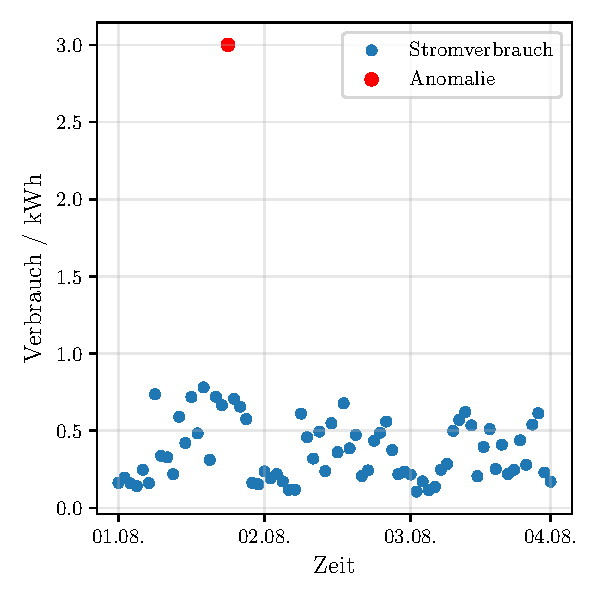
\includegraphics[width=\linewidth]{ch4_anomalien/abbildungen/punktanomalie_bsp.pdf}
        \caption{Stündliche Smart Meter Messdaten}\label{subfig:smartmeter}
    \end{subfigure}
    \begin{subfigure}[b]{0.49\linewidth}
        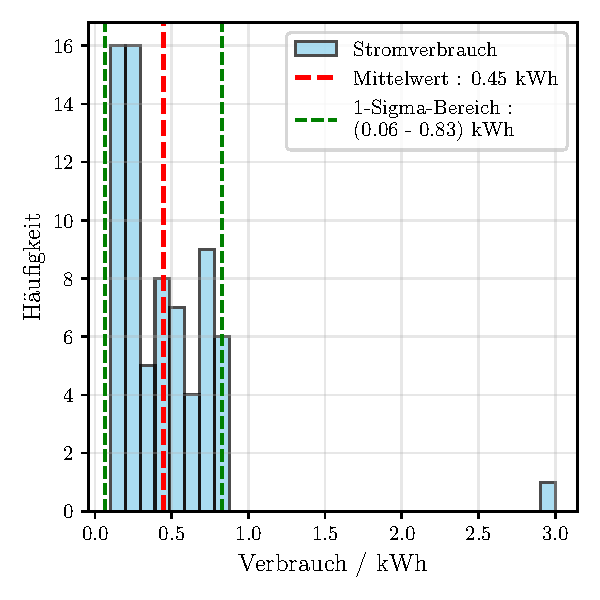
\includegraphics[width=\linewidth]{ch4_anomalien/abbildungen/punktanomalie_hist.pdf}
        \caption{\centering Histogramm des gemessenen Stromverbrauchs}\label{subfig:smartmeter_histogramm}
    \end{subfigure}
    \caption{\centering Beispielszenario einer Punktanomalie: Stromverbrauch eines Haushaltes über den Zeitraum von
    drei Tagen. Anhand des Histogramms wird die Anomalie verdeutlicht.}\label{fig:punktanomalie}
\end{figure}

Um nun eine Aussage treffen zu können, ist es wichtig, den Kontext der vorliegenden Daten zu kennen. Wenn Daten für ein weitaus größeres
Zeitfenster vorliegen, z.~B.~für eine Woche oder einen Monat, könnte sich möglicherweise zeigen, dass der hohe Verbrauch öfter und
regelmäßiger vorkommt als im gezeigten Zeitraum von drei Tagen. Ob eine globale oder lediglich eine lokale Anomalie vorliegt, wird
mit einem größeren Datensatz besser erkennbar. Die Anomalie könnte beispielsweise auf das gelegentliche Betreiben einer Sauna im Haus
zurückführbar sein, dann würde es sich lediglich um eine lokale Anomalie handeln und in einem größeren Zeitraum in bestimmten Abständen
öfter vorkommen, und wäre somit keine globale Anomalie~\Cite[Kap.~10]{Tan2014}.

Punktanomalien sind im Kontext dieser Arbeit tendenziell weniger relevant, sollen aber aufgrund ihrer grundsätzlichen Bedeutung bzgl.
Anomaliedetektion als grundlegende Kategorie trotzdem beleuchtet werden, um entsprechende Algorithmen, die der Erkennung solcher
Punktanomalien zuzuordnen sind, auch gegenüber anderen Anomalien zu testen.

\subsection{Subsequenzanomalien}

Eine Zeitserie wird gem.~\hyperref[eq:timeseries_set]{Gl.~\Ref*{eq:timeseries_set}} bereits als eine Menge definiert. Demnach wird eine
Subsequenz $S_{i,\,j} = \{\,S_i,\,\dots,\,S_j\,\}\,\subseteq\,S$ von der Zeitserie $S$ umfasst, mit der Länge oder Mächtigkeit
$|\,S_{i,\,j}\,|=j-i+1$ und $|\,S_{i,j}\,|\,\ge\,1$~\cite{Schmidl2022} und stellt somit einen Ausschnitt der urpsrünglichen Zeitserie
dar. Subsequenz\-anomalien sind Muster in Zeitreihen, die von anderen Mustern innerhalb der gleichen Zeitreihe
abweichen~\cite{Chandola2009}\Cite[S.~12]{Wenig2024}. Im Gegensatz zu Punktanomalien beziehen sich Subsequenz\-ano\-malien auf mehrere
konsekutive Datenpunkte, die ein ungewöhnliches Muster bilden. Eine anomale Subsequenz kann also bedeuten, dass die Datenpunkte innerhalb
der Subsequenz Werte in einem normalen, zu erwartenden Bereich annehmen, aber der zu Grunde liegende Trend ungewöhnlich
ist~\cite{Chandola2009}\cite[S.~17]{Boniol2021}. Solche ungewöhnlichen oder einzigartigen Trends und Entwicklungen können auf zukünftig
auftretende Probleme hindeuten, die sonst unentdeckt bleiben würden.

\begin{figure}[H]
    \centering
    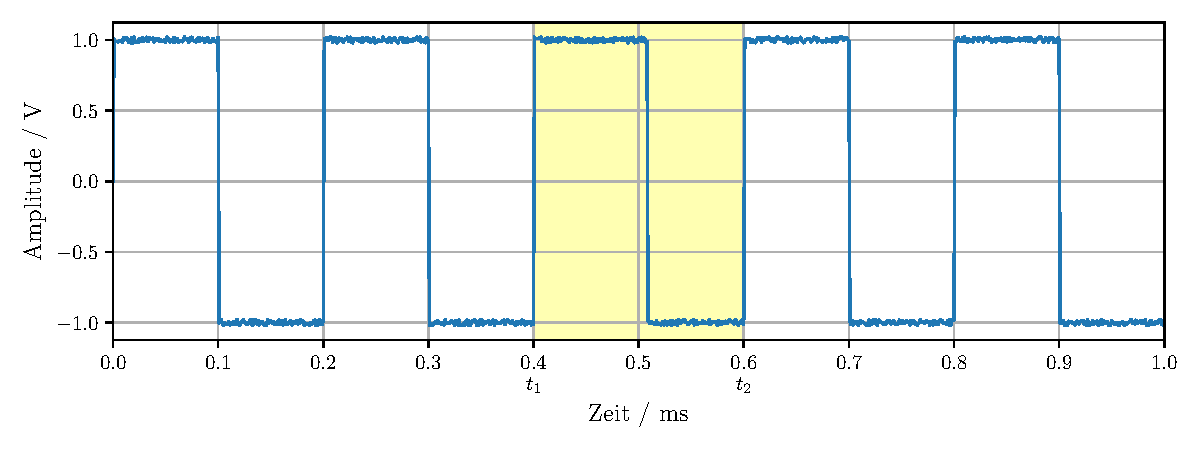
\includegraphics[width=\linewidth]{ch4_anomalien/abbildungen/subsequenz_anomalie.pdf}
    \caption{\centering Einfaches Beispiel einer Subsequenzanomalie: Rechteckspannung, die zwischen -1 und +1 V oszilliert mit einer
    Frequenz von 5 kHz. Auffällig ist die Periode zwischen $t_1=0.4\,$ms und $t_2=0.6\,$ms, bei der eine verspätete abfallende Flanke zu
    beobachten ist.}
~\label{fig:subsequenz_rect}
\end{figure}

Das Beispiel in~\hyperref[fig:subsequenz_rect]{Abb.~\Ref*{fig:subsequenz_rect}} zeigt eine sichtbare Subsequenzanomalie, die verspätete
abfallende Flanke einer gemessenen Rechteckspannung. Das Muster zwischen $t_1$ und $t_2$ ist also merklich anders verglichen zu den
restlichen 0,2 ms langen Perioden und daher eine Anomalie.

Bei der Analyse von EKG Daten spielen Subsequenzanomalien eine wichtige Rolle und können wertvolle Rückschlüsse auf die Herzgesundheit
liefern~\cite{Chuah2007}.~\hyperref[fig:ekg_herzerkrankung]{Abb.~\Ref*{fig:ekg_herzerkrankung}} zeigt EKG Daten eines Patienten mit
monomorpher ventrikulärer Tachykardie. Diese kann zu Kammerflimmern übergehen, welches unbehandelt sogar zu einem Herzstillstand
führen kann~\cite{ekgecho}\Cite[S.~131~ff.]{Davies2015}.

\begin{figure}[h]
    \centering
    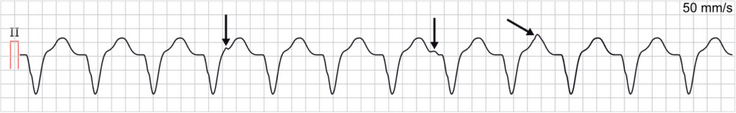
\includegraphics[width=0.85\linewidth]{ch4_anomalien/abbildungen/ventrikulaere_tachykardie.png}
    \caption{EKG Kanal mit Diagnose: Ventrikuläre Tachykardie~\cite{ekgecho}}
~\label{fig:ekg_herzerkrankung}
\end{figure}

Sichtbar sind die einzelnen Unregelmäßigkeiten im EKG Verlauf. Die Pfeile kennzeichnen die sog. P-Wellen, die Informationen darüber
liefern, dass Vorhöfe und Herzkammern nicht synchron schlagen~\cite{ekgecho}\Cite[S.~31~f.]{Davies2015}. Durch die Irregularitäten lässt
sich also erkennen, dass für den untersuchten Patienten eine Behandlung notwendig ist und betont die Wichtigkeit, diese Anomalien zu
erkennen, um wesentlich Schlimmeres zu verhindern.

Darin liegt auch eine der Herausforderungen der Subsequenzanomaliedetektion: Ab wann ist ein Trend, der so noch nicht aufgetreten ist,
Grund genug, um Maßnahmen zu ergreifen? Es bedarf also menschlicher Expertise zur Einordnung und Interpretation von Anomalien, eben wie
bei EKG Daten.

\subsection{Korrelationsanomalien}

\begin{figure}[H]
    \centering
    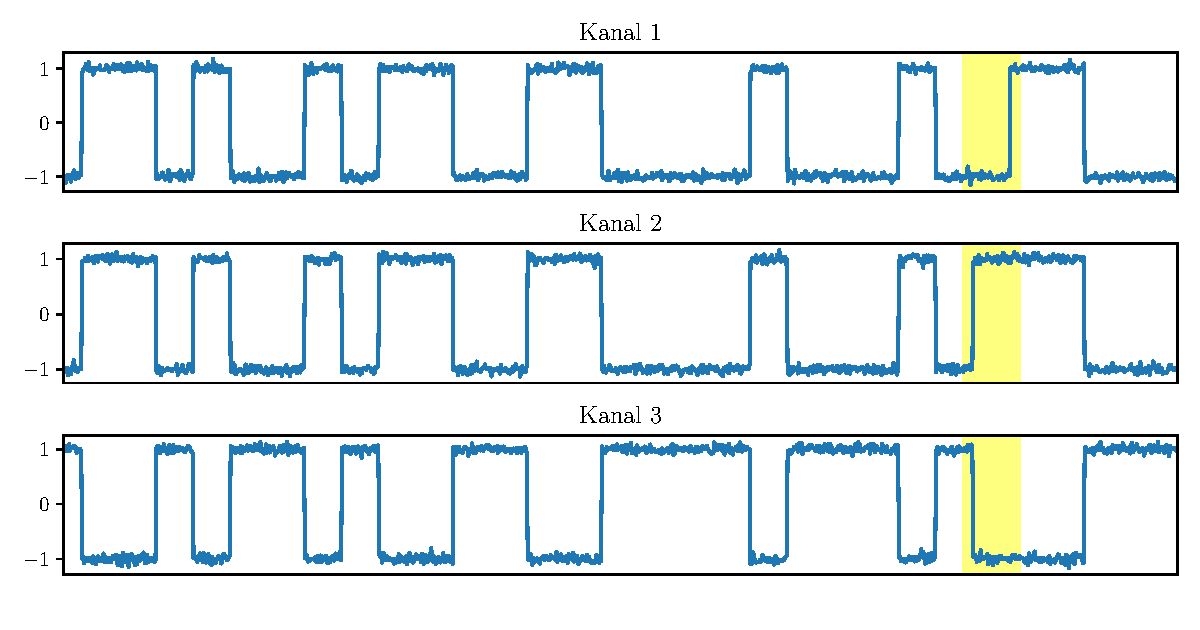
\includegraphics[width=0.95\linewidth]{ch4_anomalien/abbildungen/korrelationsanomalie.pdf}
    \caption{\centering Korrelationsanomalie zwischen Kanal 1 und den Kanälen 2 und 3 im gelb markierten Bereich. Quelle: Datensatz
        \textit{CoMuT}~\cite{NaumannCoMuT}}
~\label{fig:correlation_Anomaly}
\end{figure}

Während Punkt- und Subsequenzanomalien sowohl für univariate als auch multivariate Datensätze und Zeitserien auftreten können, sind
Korrelationsanomalien nur bei zwei oder mehr Dimensionen einer Zeitreihe möglich und betrachten die Interaktionen zwischen
verschiedenen Kanälen. Von einer Korrelationsanomalie spricht man bei Abweichungen dieser Beziehung zwischen zwei oder mehreren
Kanälen~\cite[S.12-13]{Wenig2024}~\cite{Wenig2024a}.

Im vorliegenden Beispiel in~\hyperref[fig:correlation_Anomaly]{Abb.~\Ref*{fig:correlation_Anomaly}} ist ein Auszug aus dem Datensatz
\textit{CoMuT}~- \textbf{Co}rrelated \textbf{Mu}lti\-variate \textbf{T}ime Series~\cite{NaumannCoMuT} dargestellt. Die Zeitreihe besteht
aus drei Kanälen, die zu zufälligen Zeitpunkten sprungartig ihren Wert zwischen $-$1 und 1 wechseln und jeweils leicht verrauscht sind.
Kanal 1 und 2 sind stark korreliert, während Kanal 3 stark antikorreliert zu den beiden ersten Kanälen ist. Diese Korrelation wird im
markierten Bereich verletzt, da Kanal 1 zeitlich versetzt zu den anderen beiden Kanälen springt~$-$~somit liegt eine
Korrelations\-anomalie vor.

\section{Algorithmen zur Anomaliedetektion}\label{sec:algorithmen}
In der Literatur gibt es eine breite Spanne an erprobten, möglichen Algorithmen zur Detektion der gesuchten
Anomalietypen~\cite{Schmidl2022}~\cite{BlazquezGarcia2020}~\cite{Mane2022}~\cite{Wenig2024a}. Da der zeitliche Rahmen dieser Arbeit
begrenzt ist und der vorrangige Fokus die Anwendung der Anomaliedetektionsthematik ist, müssen bei der Auswahl der Algorithmen
einige Einschränkungen vorab festgelegt werden. Dazu gehört, dass ein Algorithmus bereits implementiert wurde und optimalerweise als Open
Source Python Bibliothek o.ä.~zur Verfügung steht oder die Idee durch bereits vorhandene Komponenten einfach selbst implementiert
werden kann. Desweiteren soll es sich zu Beginn um Algorithmen handeln, die ohne vorheriges Training
auskommen, also sog. Unsupervised Learning Algorithmen. Dazu eignen sich die folgenden Techniken bzw.~Algorithmen am Besten.

\subsection{Histogram-Based Outlier Score}
Der erste Algorithmus zur Detektion von Punktanomalien ist der zur Ermittlung des \textbf{Histogram-Based Outlier Score} (HBOS), der sich
sowohl für univariate als auch multivariate Zeitserien eignet. Dabei wird für jede Dimension eine Analyse der Häufigkeitsverteilung per
Histogramm durchgeführt und anhand dessen der namensgebende Outlier Score berechnet. Die Häufigkeit aller Werte innerhalb eines Bins wird als
Dichte aufsummiert, und die Dichte ergibt gem.~\hyperref[eq:hbos]{Gl.~\Ref*{eq:hbos}} invers logarithmiert den Outlier Score. So erhalten Bins
mit geringen Häufigkeiten, also die Bins mit selten auftretenden Werten~-~wahrscheinliche Anomalien~-~einen hohen Outlier Score und können
so als Anomalie detektiert werden~\cite{Goldstein2012}.

\begin{equation}
    \text{HBOS}\,(p)\, =\, \sum_{i=0} ^ {d}\, \log \left( \frac{1}{\text{hist}_i(p)} \right)
\label{eq:hbos}
\end{equation}

Die Häufigkeitsanalyse über den kompletten Datensatz bzw.~eine sehr große Datenmenge führt dazu, dass lokale Anomalien nicht erkannt werden,
da diese Werte trotzdem innerhalb der erwarteten Verteilung liegen und im globalen Kontext nicht herausstehen,
wie~\hyperref[fig:hbos_lokale_probleme]{Abb.~\Ref*{fig:hbos_lokale_probleme}} zeigt. Einfache Abhilfe liefert die
in~\hyperref[fig:hbos_lösung]{Abb.~\Ref*{fig:hbos_lösung}} dargestellte Erweiterung um ein gleitendes Fenster variabler Größe. Der HBOS wird dann innerhalb
eines jeden Fensters ermittelt, wodurch der zeitliche Kontext mit einbezogen wird und auch lokale Anomalien erkannt werden. Multivariate Systeme
können ebenfalls einfach analysiert werden, indem für jede Variable oder Dimension separate Histogramme erstellt werden.

\begin{figure}[H]
    \centering
        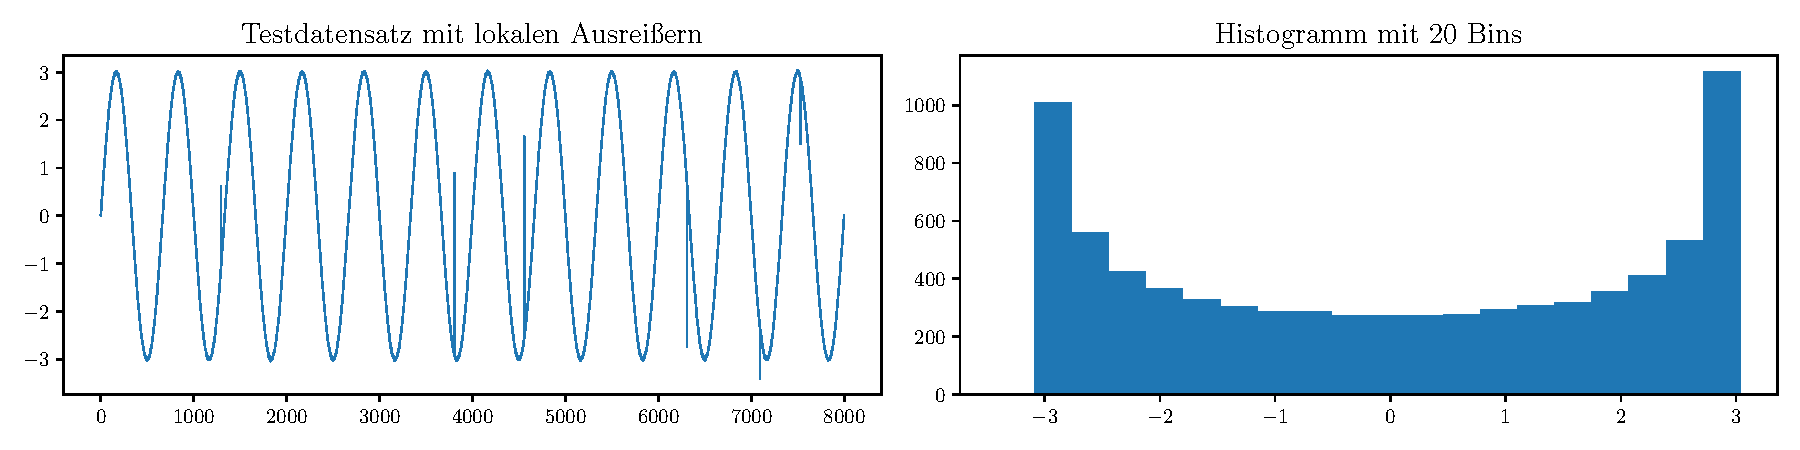
\includegraphics[width=1\linewidth]{ch4_anomalien/abbildungen/hbos_lokal_problem.pdf}    
    \caption{\centering Problematik der Detektion lokaler Punktanomalien: Da lokale Anomalien innerhalb des erwarteten Wertebereichs und damit der erwarteten
    Verteilung liegen, werde diese vom Algorithmus nicht als Ausreißer erkannt.}
~\label{fig:hbos_lokale_probleme}
\end{figure}

\begin{figure}[H]
    \centering
        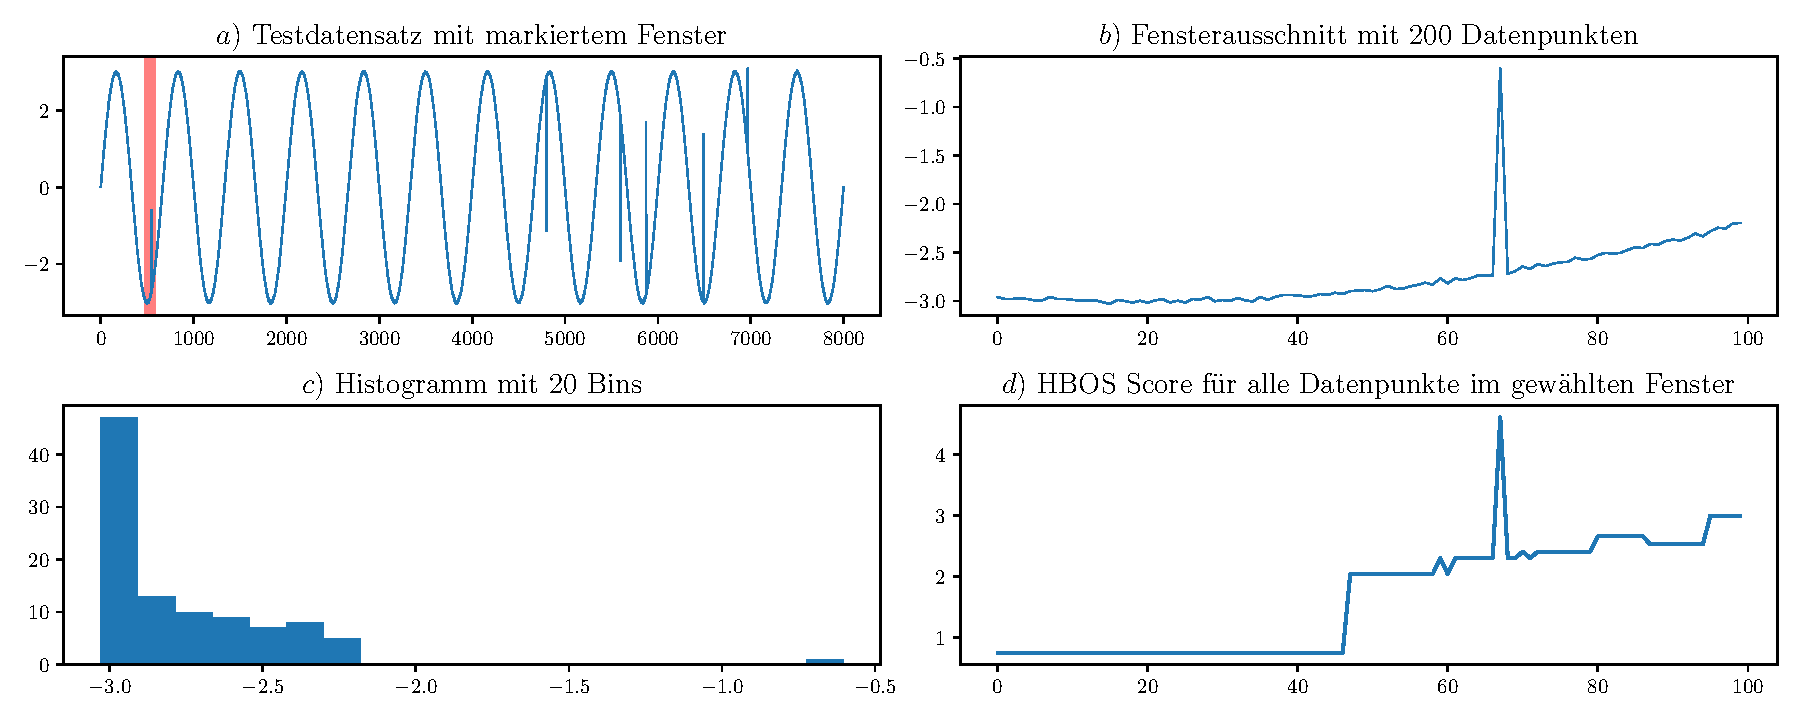
\includegraphics[width=1\linewidth]{ch4_anomalien/abbildungen/hbos_lokale_anomalien.pdf}    
    \caption{\centering Lösung der Detektionsproblematik für lokale Anomalien durch ein gleitendes Fenster. Beispielhaft dargestellt an einer Fenstergröße
    von $n=100$.}
~\label{fig:hbos_lösung}
\end{figure}

\subsection{Sliding Window Z-Score}
Durch die Berechnung eines gleitenden Mittelwerts sowie der entsprechenden gleitenden Standardabweichung kann der Z-Score eines Datenpunkts
gem.~\hyperref[eq:zscore]{Gl.~\Ref*{eq:zscore}} bestimmt werden. Der Z-Score wird in einer ähnlichen Form bereits im Jahre 1969 in \textit{Grubb's
Test} erstmals erwähnt~\cite{Grubbs1969}. Dabei bezeichnet $x_i$ den zu untersuchenden Datenpunkt, $\mu_W$ den Mittelwert und $\sigma_W$ die
Standardabweichung des Fensters~\Cite[S.~15:31]{Chandola2009}.

\begin{equation}
    Z_i\, =\, \frac{|\, x_i\,-\, \mu_W\,|}{\sigma_W}
\label{eq:zscore}
\end{equation}

Um für die Zeitserie den Zeitbezug beizubehalten, werden die statistischen Größen mit einem gleitenden Fenster berechnet, um auch lokale Ausreißer,
deren absolute Werte innerhalb der globalen Verteilung liegen, detektieren zu können. Dabei ist die Fenstergröße zunächst fest. Entsprechend des
Z-Scores deutet ein hoher Wert auf eine Anomalie hin, aufgrund der großen Abweichung zum gleitenden Mittelwert trotz Skalierung durch die
Standardabweichung. Damit ist der Z-Score eine dimensionslose Größe, die direkt als Anomaly Score interpretiert werden kann.

\subsection{GrammarViz 2.0}
Der nächste Algorithmus namens \textbf{GrammarViz} wird zur Detektion von Subsequenzanomalien eingesetzt~\cite{Senin2015}. Die Funktionsweise
basiert auf der Diskretisierung einer Zeitreihe in Symbole. Für Subsequenzen unterschiedlicher Größe wird dann versucht, diese mit
Grammatikregeln zu beschreiben. Kann sich eine Subsequenz nicht entsprechend der am häufigsten auftretenden Grammatikregeln charakterisieren
lassen, so handelt es sich wahrscheinlich um eine anomale Sequenz, beispielsweise durch ein ungewöhnliches Muster oder eine neue Trendentwicklung.

Da zum Erlernen von Grammatikregeln diskretisierte Daten benötigt werden, erfolgt die Diskretisierung in einem ersten Schritt mit dem Algorithmus SAX
(\textit{\textbf{S}ymbolic \textbf{A}ggregation Appro\textbf{X}imation}), der aus Datensätzen bzw.~-sequenzen äquivalente Symbole erzeugt~\cite{Patel}.
Aufgrund der Natur von Subsequenzanomalien wird SAX per gleitendem Fenster angewandt. Innerhalb jedes Fensters wird die Subsequenz Z-normalisiert (vgl.
Z-Scoring in~\hyperref[eq:zscore]{Gl.~\Ref*{eq:zscore}}) und anschließend in $w$ gleichwahrscheinliche Segmente diskretisiert, mit $w$ als Anzahl an
Symbolen. Durch die Z-Normalisierung folgt die Sequenz einer Gauß-Verteilung und wird
entspr.~\hyperref[tab:normalverteilung_segmente]{Tab.~\Ref*{tab:normalverteilung_segmente}} sowie am Beispiel $w=6$
in~\hyperref[fig:normalverteilung_segmente]{Abb.~\Ref*{fig:normalverteilung_segmente}} unterteilt.

\begin{table}[H]
    \centering
    \renewcommand{\arraystretch}{1.1}
    \begin{tabular}{l|rrrrrrrr}
        \backslashbox{$\beta _i$}{$w$} & 3                 & 4                   & 5                   & 6                   & 7                   & 8                   & 9                   & 10      \\
    \hline
    $\beta _1$ & $-0,43$             & $-0,67$             & $-0,84$             & $-0,97$             & $-1,07$             & $-1,15$             & $-1,22$             & $-1,28$ \\
    $\beta _2$ & $0,43$              & 0                   & $-0,25$             & $-0,43$             & $-0,57$             & $-0,67$             & $-0,76$             & $-0,84$ \\
    $\beta _3$ & \cellcolor{blue!15} & $0,67$              & $0,25$              & 0                   & $-0,18$             & $-0,32$             & $-0,43$             & $-0,52$ \\
    $\beta _4$ & \cellcolor{blue!15} & \cellcolor{blue!15} & $0,84$              & $0,43$              & $0,18$              & 0                   & $-0,14$             & $-0,25$ \\
    $\beta _5$ & \cellcolor{blue!15} & \cellcolor{blue!15} & \cellcolor{blue!15} & $0,97$              & $0,57$              & $0,32$              & $0,14$              & 0       \\
    $\beta _6$ & \cellcolor{blue!15} & \cellcolor{blue!15} & \cellcolor{blue!15} & \cellcolor{blue!15} & $1,07$              & $0,67$              & $0,43$              & $0,25$  \\
    $\beta _7$ & \cellcolor{blue!15} & \cellcolor{blue!15} & \cellcolor{blue!15} & \cellcolor{blue!15} & \cellcolor{blue!15} & $1,15$              & $0,76$              & $0,52$  \\
    $\beta _8$ & \cellcolor{blue!15} & \cellcolor{blue!15} & \cellcolor{blue!15} & \cellcolor{blue!15} & \cellcolor{blue!15} & \cellcolor{blue!15} & $1,22$              & $0,84$  \\
    $\beta _9$ & \cellcolor{blue!15} & \cellcolor{blue!15} & \cellcolor{blue!15} & \cellcolor{blue!15} & \cellcolor{blue!15} & \cellcolor{blue!15} & \cellcolor{blue!15} & $1,28$ 
    \end{tabular}
\caption{\centering z-Werte einer Normalverteilung für Segmente mit gleichem Flächeninhalt ergo gleicher Wahrscheinlichkeit. $\beta _i$ mit
$1 \le i \le w-1$ sowie $\beta _0=-\infty$ und $\beta _w=+\infty$ entsprechen den z-Koordinaten für die jeweilige Aufteilung der z-Achse.
Quelle:~\cite{Patel}}
~\label{tab:normalverteilung_segmente}
\end{table}

\begin{figure}[t!]
    \centering
        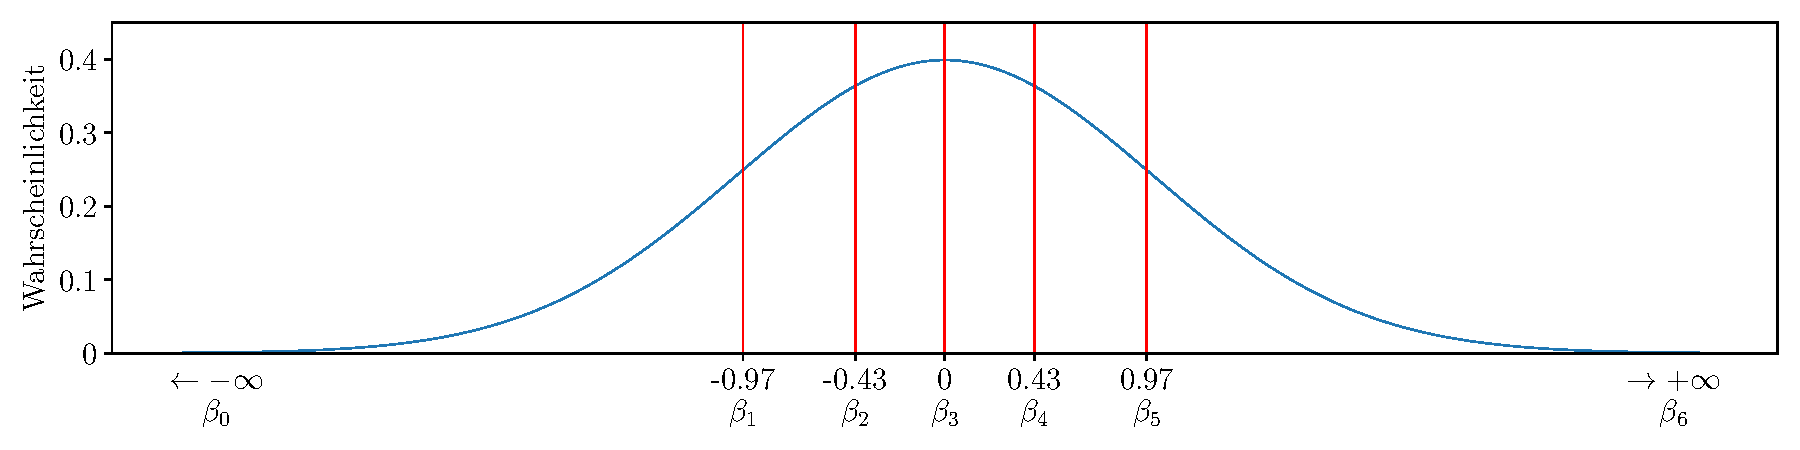
\includegraphics[width=\linewidth]{ch4_anomalien/abbildungen/normalverteilung_SAX_segmente.pdf}
    \caption{Normalverteilung mit $w=6$ gleichwahrscheinlichen Segmenten gem.~\hyperref[tab:normalverteilung_segmente]{Tab.~\Ref*{tab:normalverteilung_segmente}}}
~\label{fig:normalverteilung_segmente}
\end{figure}

Die diskretisierte Subsequenz produziert dann eine Menge an SAX Worten, die mit dem Grammatikinferenzalgorithmus Sequitur~\cite{NevillManning1997}
weiterverarbeitet werden, um rekursiv kontextfreie Grammatikregeln aufzustellen. Mithilfe einer GUI kann ein Datensatz analysiert werden und mit der
erzeugten \textbf{Rule Density Curve} sowie den einzeln aufgelisteten potenziell anomalen Sequenzen untersucht werden. Die Rule Density Curve gibt Aufschluss
darüber, wieviele Grammatikregeln pro Datenpunkt greifen. Das heißt anschaulich: je mehr Grammatikregeln einer Subsequenz zugeschrieben werden können, desto normaler
ist ein Datenpunkt bzw.~eine Subsequenz~\cite{senin-gv2}.

\subsection{Sliding Window Isolation Forest Density}
\label{subsec:swifd}

\begin{figure}[b!]
    \centering
    \begin{tikzpicture}
        \node[anchor=south west,inner sep=0] (image) at (0,0) {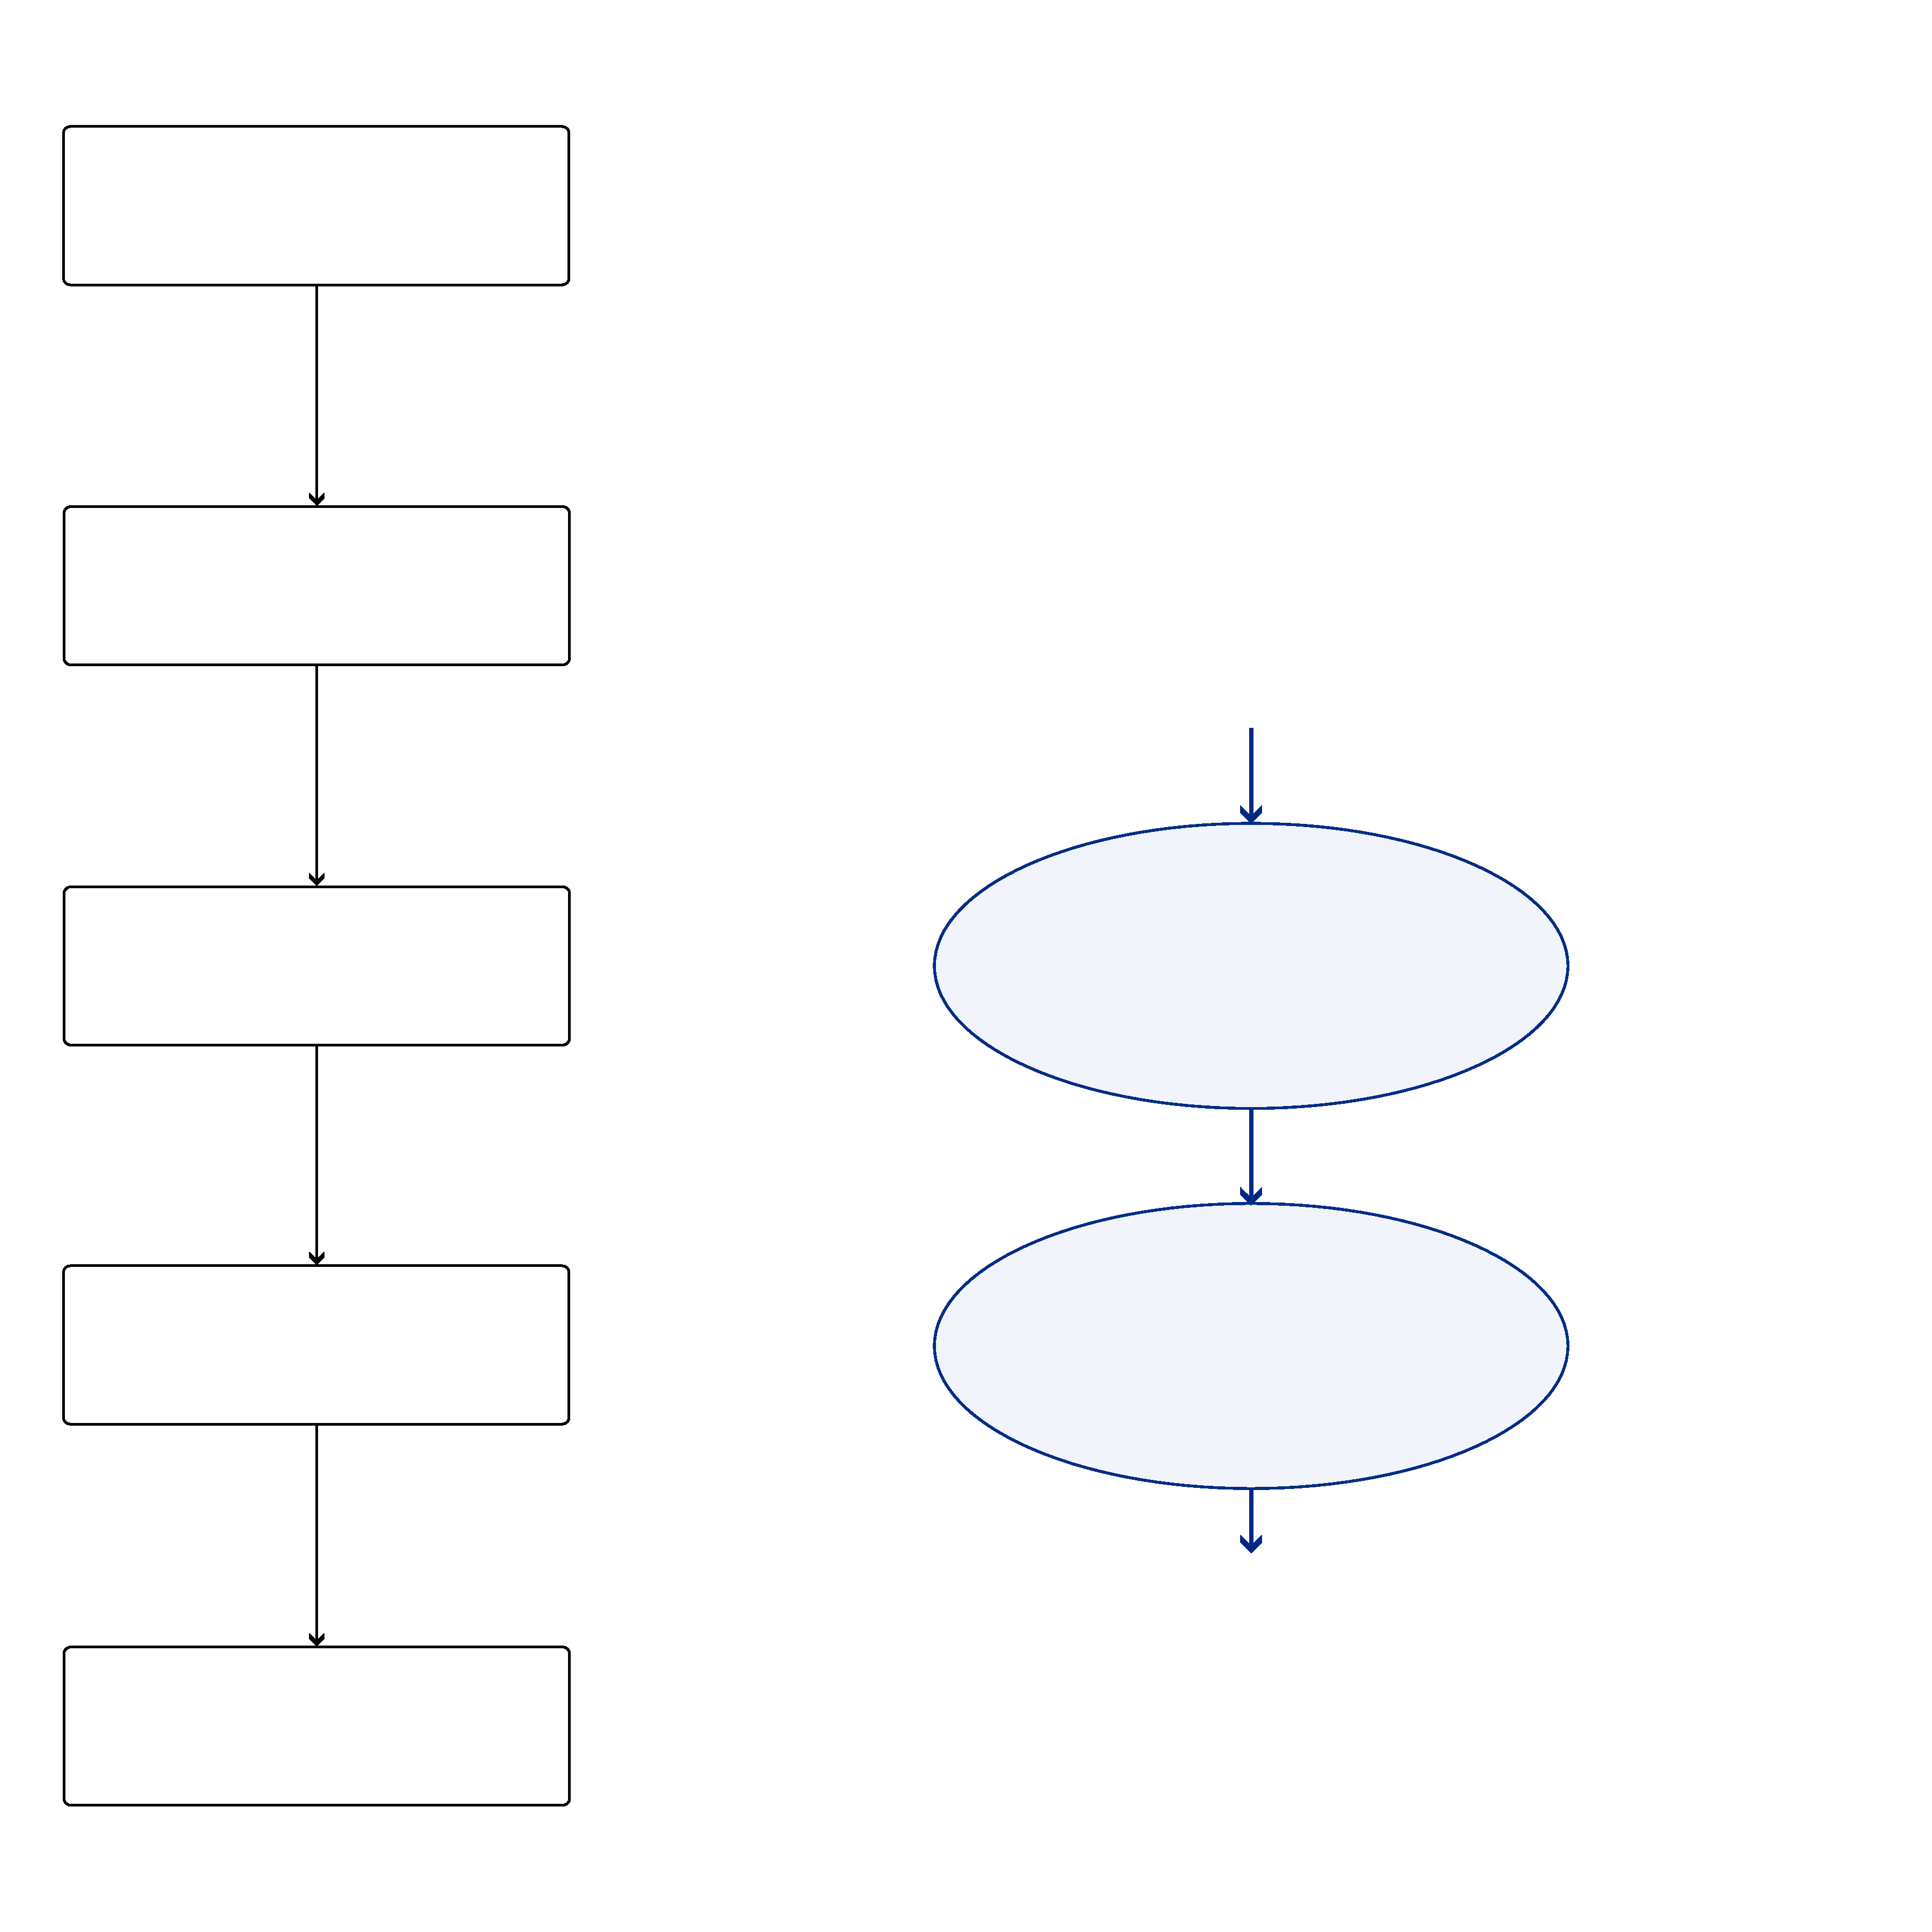
\includegraphics[width=1\linewidth]{ch4_anomalien/abbildungen/vorlage_SWIFD_schema.pdf}};
        \begin{scope}[x={(image.south east)},y={(image.north west)}]
            \node at (0.16,0.89) {\large \parbox{4cm}{\centering \textbf{Eingangssignal}:\\Zeitserie}};
            \node at (0.65,0.89) {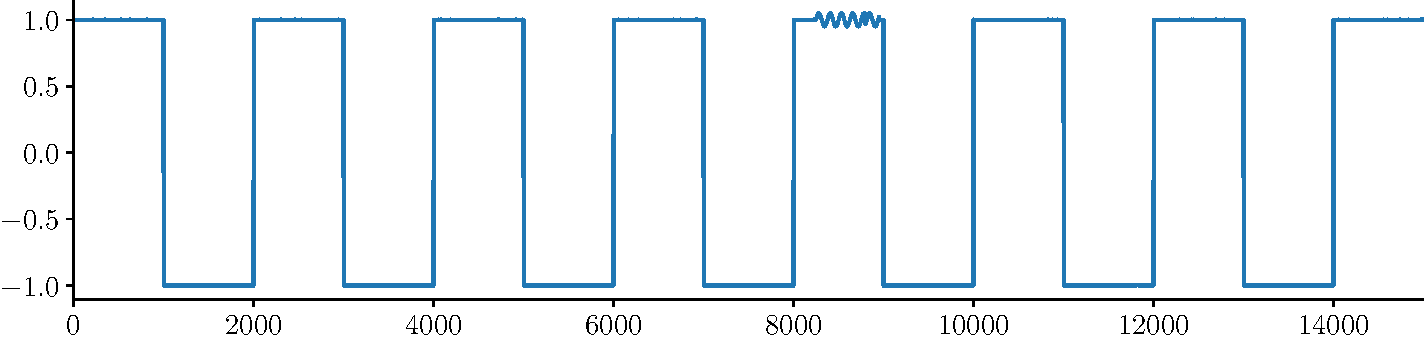
\includegraphics[width=0.68\linewidth]{ch4_anomalien/abbildungen/noisy_square_wave.pdf}};
            \node at (0.16,0.695) {\large \parbox{4cm}{\centering \textbf{1. Schritt}:\\Feature Matrix}};
            \node at (0.622,0.695) {
                    \begin{tikzpicture}
                        \node at (0,1) {$F = \begin{pmatrix} 
                            \mu_{0} & \mu_{1} & \dots & \mu_{_n-1} \\
                            \sigma_{0} & \sigma_{1} & \dots & \sigma_{_n-1} \\
                            \text{min}_{0} & \text{min}_{1} & \dots & \text{min}_{n-1} \\
                            \text{max}_{0} & \text{max}_{1} & \dots & \text{max}_{n-1} \\
                        \end{pmatrix}$};
                    \end{tikzpicture}
            };
            \node at (0.16,0.5) {\large \parbox{4cm}{\centering \textbf{2. Schritt}:\\Isolation Forest}};
            \node at (0.65,0.5) {\large \parbox{4cm}{\centering \textbf{Anomalien in Feature Matrix finden}}};
            \node at (0.16,0.305) {\large \parbox{4cm}{\centering \textbf{3. Schritt}:\\Anomalien abtragen}};
            \node at (0.65,0.305) {\large \parbox{4cm}{\centering \textbf{Für alle Fenstergrößen aufsummieren}}};
            \node at (0.16,0.11) {\large \parbox{4.2cm}{\centering \textbf{4. Schritt}:\\Dichtekarte berechnen}};
            \node at (0.65,0.11) {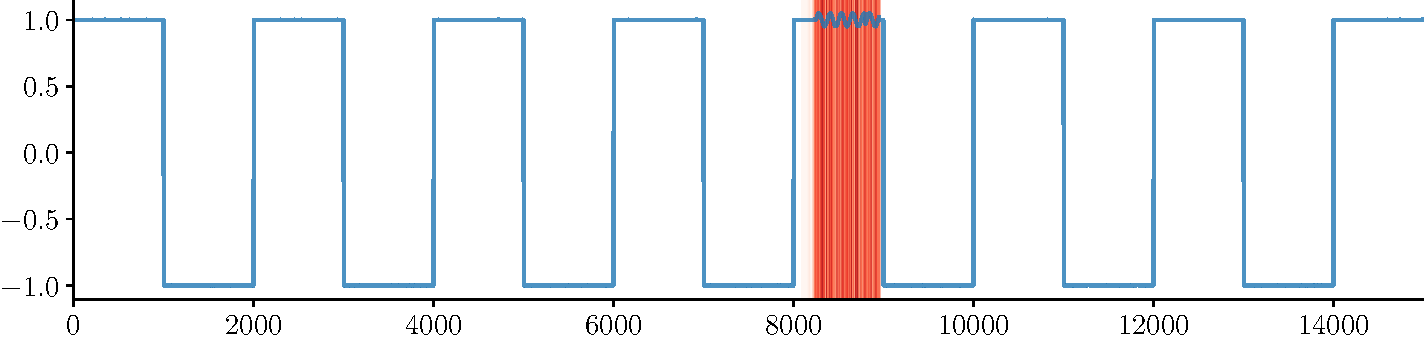
\includegraphics[width=0.68\linewidth]{ch4_anomalien/abbildungen/SWIFD_heatmap.pdf}};
        \end{scope}
    \end{tikzpicture}
    \caption{Schematischer Ablauf des SWIFD Algorithmus}
~\label{fig:swifd_schema}
\end{figure}

Der Algorithmus namens \textbf{Sliding Window Isolation Forest Density}~-~kurz \textbf{SWIFD}~-~dient der Anomalieerkennung in Zeitreihen durch die Berechnung einer
Anomaliedichtekarte mittels des Isolation Forest-Verfahrens~\cite{Liu2012}. Der schematische Ablauf ist dabei~\hyperref[fig:swifd_schema]{Abb.~\Ref*{fig:swifd_schema}}
zu entnehmen. Zunächst werden aus der Zeitreihe über gleitende Fenster statistische Merkmale
extrahiert. Hierzu wird die Zeitreihe segmentiert, wobei jedes Fenster durch Mittelwert, Standardabweichung, Minimum und Maximum beschrieben wird. Die
Fenstergröße wird aus einer vordefinierten Menge gewählt, wobei sich die Schrittweite in Abhängigkeit der Fenstergröße ergibt.

Die so gewonnenen Merkmalsvektoren werden anschließend mit dem Isolation Forest-Algorithmus verarbeitet, der auf der Grundidee von Liu et al.~\cite{Liu2012}
basiert und um die gleitenden Fenster von Ding et al.~\cite{Ding2013} weiterentwickelt wurde. Dieser konstruiert Entscheidungsbäume, in denen isolierte
Datenpunkte~–~also potenzielle Anomalien~–~mit kürzeren Pfaden identifiziert werden als
reguläre Datenpunkte. Während herkömmliche Isolation-Forest-Ansätze binäre Entscheidungen über Anomalien treffen, integriert SWIFD eine Dichtebetrachtung.
Anstatt einzelne Punkte als Anomalien zu markieren, wird für jedes Fenster ein Dichtewert berechnet, indem erkannte Anomalien aufsummiert werden.

Um lokale Schwankungen zu glätten und die visuelle Interpretierbarkeit zu verbessern, erfolgt abschließend eine Glättung der Anomaliedichte mithilfe eines
Gaußschen Filters. Dieser Ansatz kombiniert somit die Effizienz von Isolation Forest mit einer kontinuierlichen Dichteschätzung, wodurch nicht nur isolierte
Anomalien erkannt, sondern auch Bereiche mit einer erhöhten Anomaliewahrscheinlichkeit identifiziert werden können. Dies ist besonders nützlich für die
Analyse von Zeitreihen mit strukturellen Veränderungen, bei denen einzelne Punktanomalien möglicherweise nicht ausreichen, um ein klares Bild der zugrunde
liegenden Muster zu liefern.

\subsection{Mahalanobis-Distanz mit SWIFD}
Der Algorithmus \textbf{Mahalanobis-Distanz mit SWIFD}~-~kurz \textbf{MD-SWIFD}~-~wird zur Detektion von Korrelationsanomalien eingesetzt und kombiniert zwei
wesentliche Konzepte: die Mahala\-nobis-Distanz und Isolation Forest, wie er in~\hyperref[subsec:swifd]{Abs.~\Ref*{subsec:swifd}} bereits
zur Subsequenzanomaliedetektion angewandt wird. Die Weiterentwicklung um die Mahalanobis-Distanz ermöglicht die Erkennung von Anomalien in der Korrelation
in multivariaten Zeitserien~\cite{McLachlan1999}.

Als eine Erweiterung der euklidischen Distanz wird die Mahalanobis in multivariaten Datensätzen verwendet, um die Entfernung eines Punktes von einem Mittelwert unter
Berücksichtigung der Korrelationen zwischen den Dimensionen zu messen. Für einen Punkt $x$ in einer multivariaten Zeitserie, den Mittelwert $\mu$ und die
Kovarianzmatrix $\Sigma$, wird die Mahalanobis-Distanz $D_M$ wie folgt berechnet:

\begin{equation}
    D_M(x)\, = \sqrt{{\left( x\,-\,\mu \right)}^T\, \Sigma^{-1}\,(x\,-\,\mu)}
\label{eq:mahalanobis_dist}
\end{equation}

\begin{figure}[t!]
    \centering
    \begin{tikzpicture}
        \node[anchor=south west,inner sep=0] (image) at (0,0) {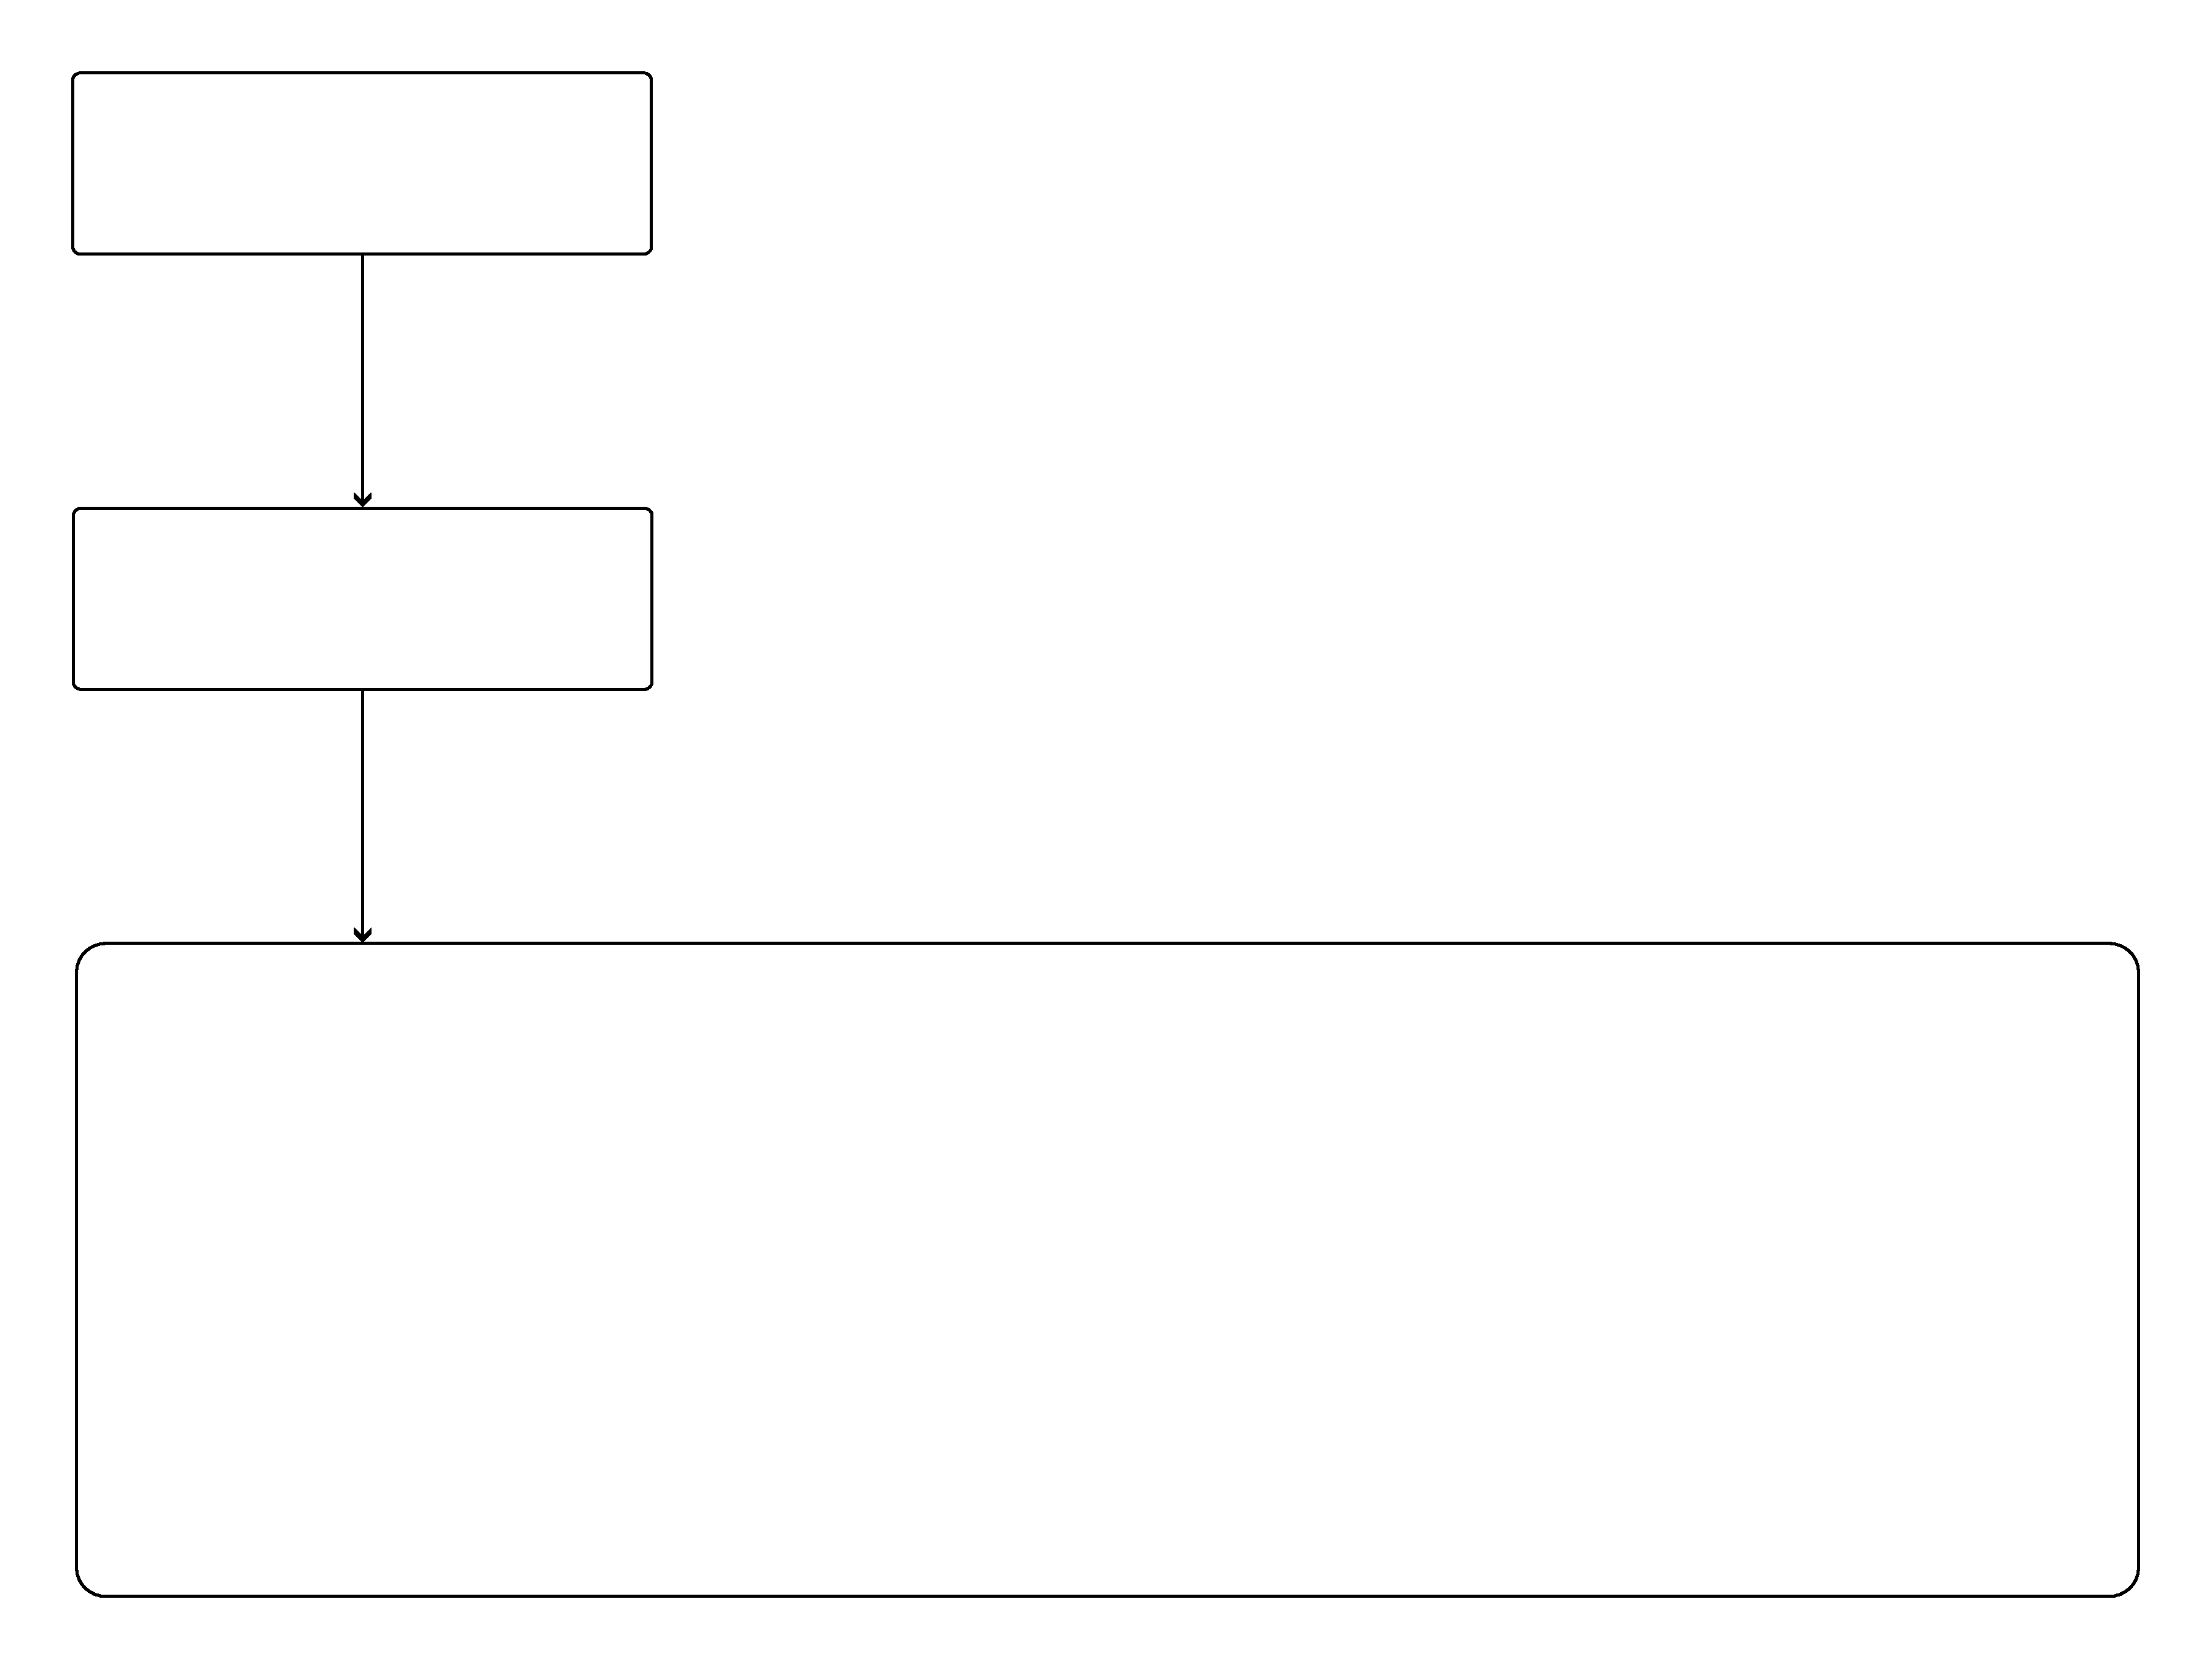
\includegraphics[width=1\linewidth]{ch4_anomalien/abbildungen/vorlage_MD-SWIFD_schema.pdf}};
        \begin{scope}[x={(image.south east)},y={(image.north west)}]
            \node at (0.16,0.9) {\large \parbox{4cm}{\centering \textbf{Eingangssignal}:\\Zeitserie}};
            \node at (0.65,0.76) {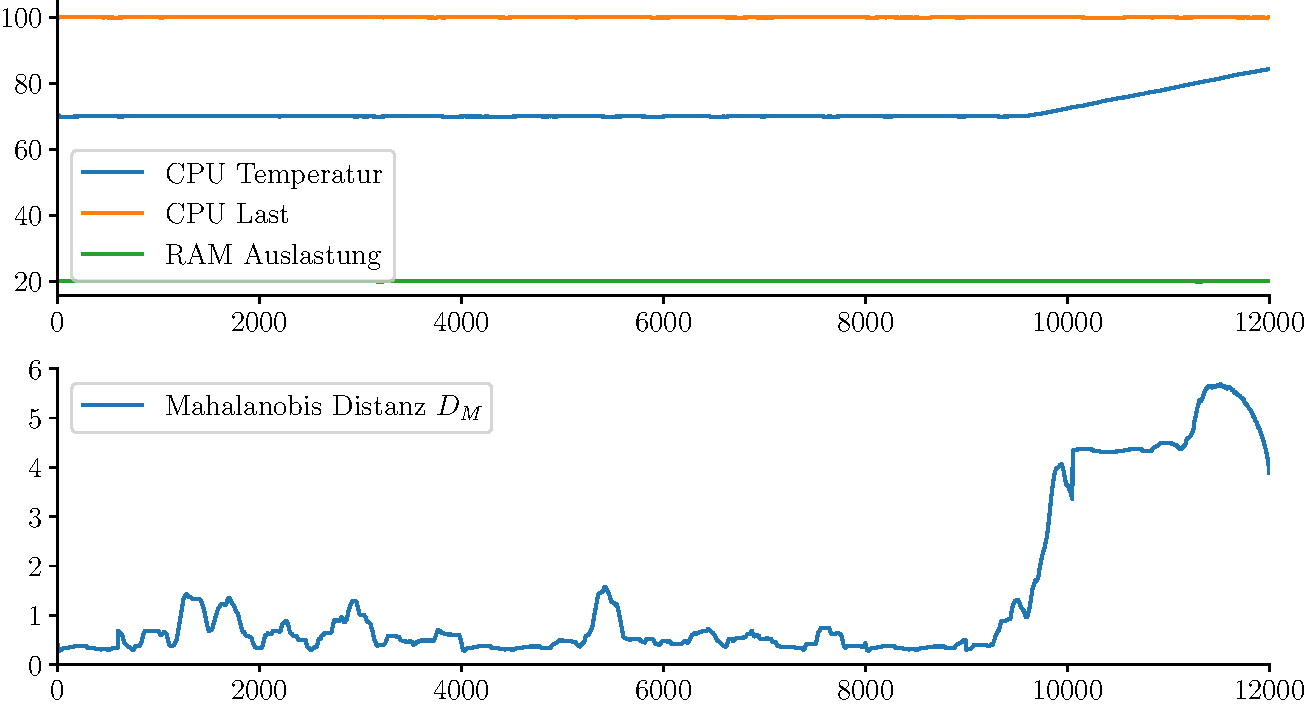
\includegraphics[width=0.68\linewidth]{ch4_anomalien/abbildungen/combined_plots.pdf}};
            \node at (0.16,0.645) {\large \parbox{4cm}{\centering \textbf{1. Schritt}:\\Mahalanobis Distanz}};
            \node at (0.5,0.39) {\large \parbox{8cm}{\centering \textbf{alle weiteren Schritte}:\\identisch zu SWIFD}};
            \node at (0.5,0.2) {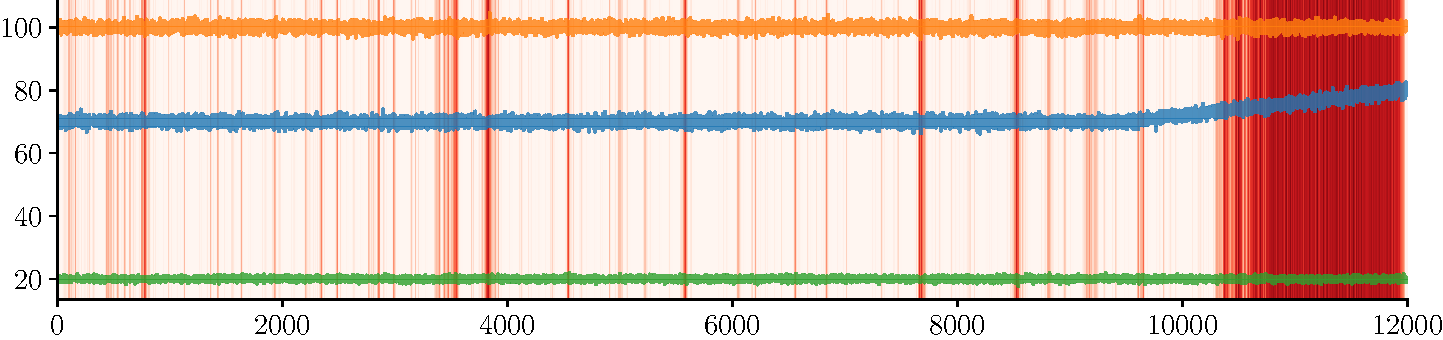
\includegraphics[width=0.9\linewidth]{ch4_anomalien/abbildungen/md_swifd_result_schema.pdf}};
        \end{scope}
    \end{tikzpicture}
    \caption{Schematischer Ablauf des MD-SWIFD Algorithmus als Erweiterung von SWIFD}
~\label{fig:md_swifd_schema}
\end{figure}

In Verbindung mit SWIFD wird der \glqq zeitliche Verlauf\grqq~der Mahalanobis Distanz~-~also die
Mahalanobis Distanz, die zu jedem Zeitstempel der Zeitserie korrespondiert~-~als Analysesignal verwendet. In der Mahalanobis-Distanz stecken sämtliche
Informationen über das Korrelationsverhalten der Zeitserie und so können am Verlauf der Distanz Anomalien detektiert werden.

MD-SWIFD macht sich also die Funktionalität von SWIFD zu Nutze und kann so in der weiterentwickelten Version Anomalien in der Korrelation mehrerer Variablen
zuverlässig detektieren.

\subsection{Elliptic Envelope Ansatz}
Unter der Annahme, dass Daten einer multivariaten Normalverteilung folgen, wird der Elliptic Envelope verwendet, um Ausreißer in einem Datensatz zu
identifizieren. Der Algorithmus geht davon aus, dass die Mehrheit der Datenpunkte innerhalb einer elliptischen Region um den Mittelpunkt der Verteilung
liegt. Ziel des Verfahrens ist es, eine elliptische Grenze zu bestimmen, die die zentrale Datenverteilung beschreibt. Punkte, die außerhalb dieser Grenze
liegen, gelten als Ausreißer.

\begin{figure}[t!]
    \centering
        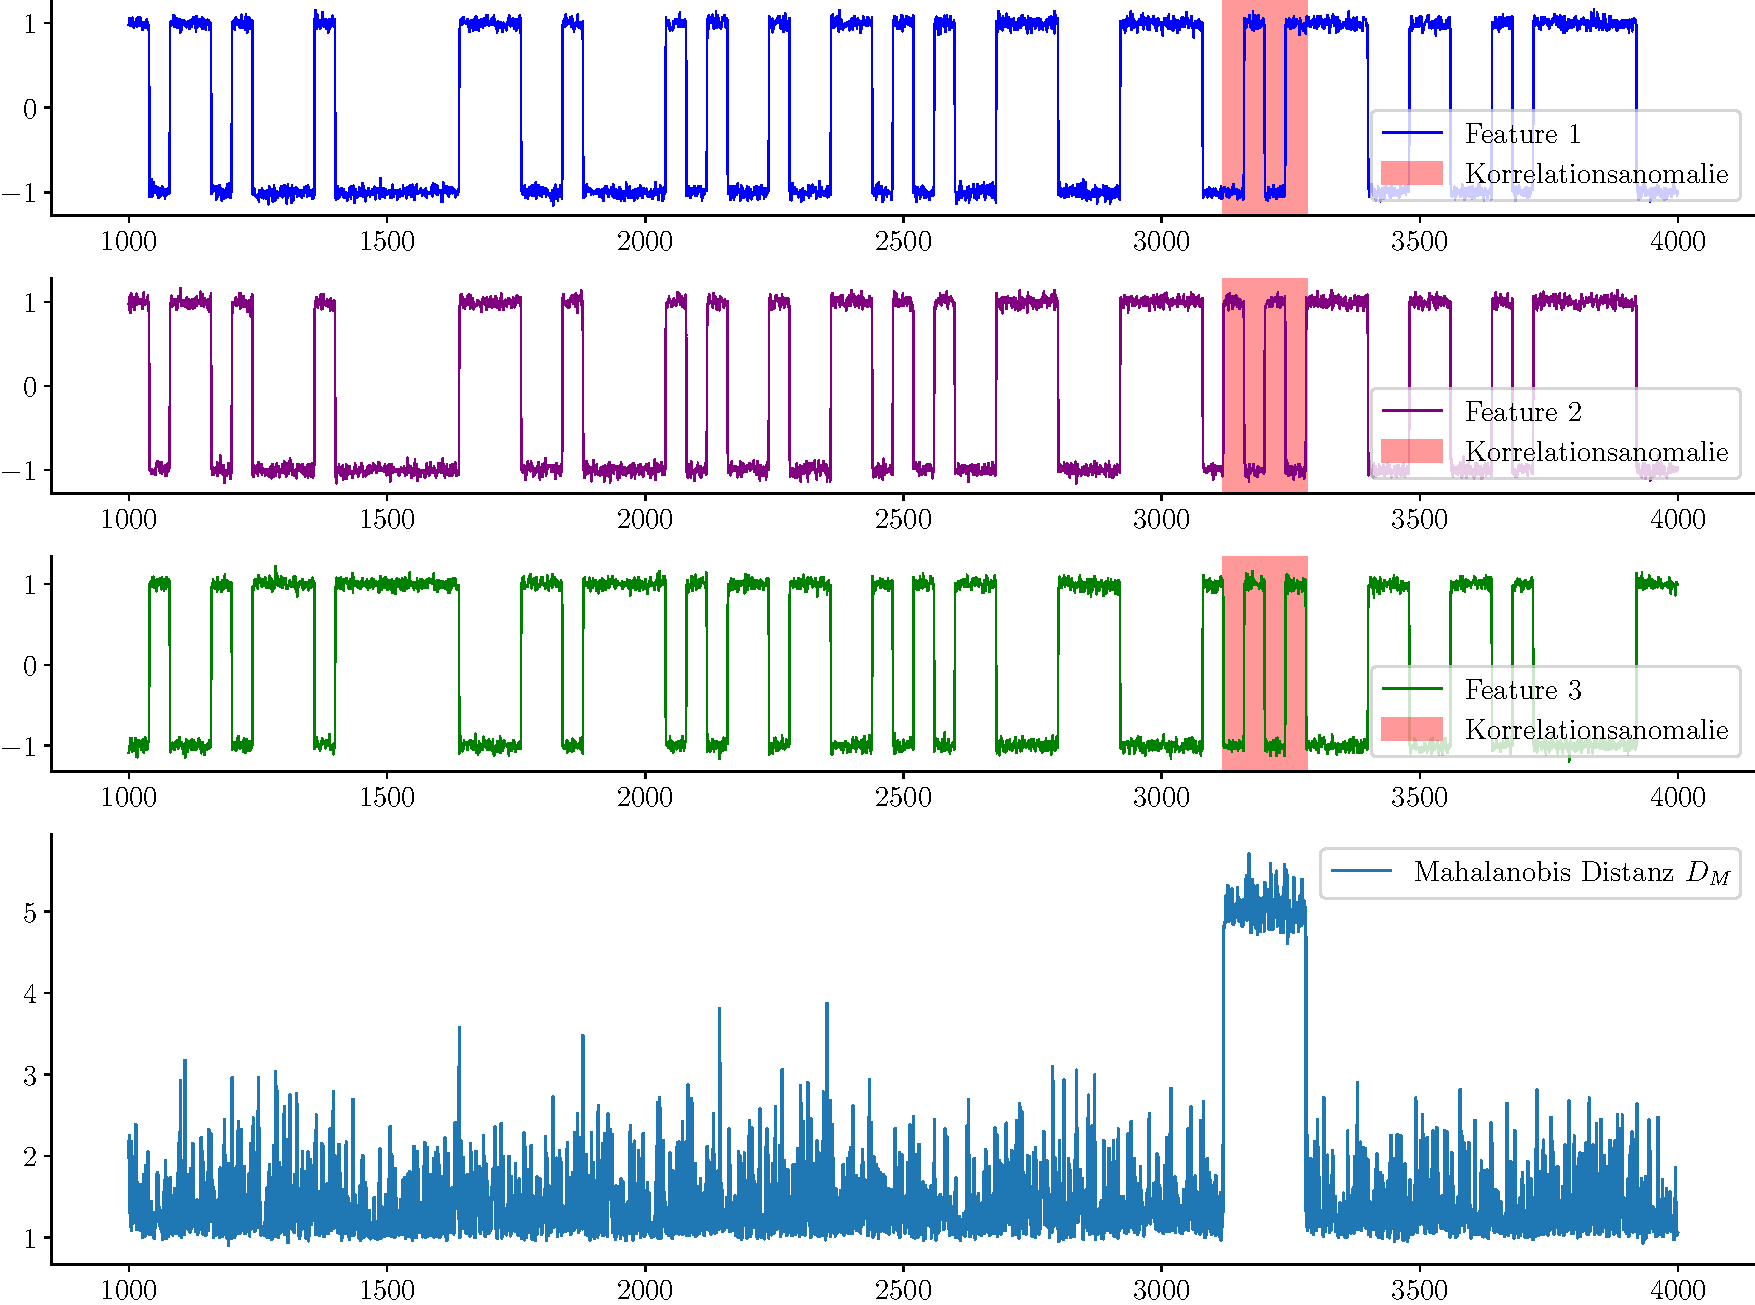
\includegraphics[width=1\linewidth]{ch4_anomalien/abbildungen/EE_mahalanobis.pdf}
    \caption{Ausschnitt aus dreidimensionaler Zeitreihe mit entsprechender Mahalanobis Distanz $D_M$. Anhand von $D_M$ können Korrelationsanomalien
        durch Setzen eines Schwellwerts erkannt werden, wenn die Distanz oberhalb dieser Schwelle liegt.}
\label{fig:EE_mahalanobis}
\end{figure}

Die Funktionsweise des Elliptic Envelope basiert auf der Schätzung der Kovarianzmatrix der Daten und der Bestimmung einer Ellipse, die diese am besten
beschreibt. Mithilfe des Maximum-Likelihood-Verfahrens wird die multivariate Normalverteilung ermittelt, die die größten Anteile der Daten umfasst. Die
Hauptachsen dieser Ellipse werden durch die Eigenwerte und Eigenvektoren der Kovarianzmatrix bestimmt. Um Ausreißer zu erkennen, wird eine
Mahalanobis-Distanz berechnet, und Datenpunkte, die eine zu hohe Distanz aufweisen, werden als Anomalien identifiziert~\cite{Ashrafuzzaman2020}.

Der Elliptic Envelope wird häufig in Bereichen eingesetzt, in denen die Annahme einer Normalverteilung zutrifft, wie beispielsweise in der Analyse von
verdächtigen Netzwerkaktivitäten~\cite{Ashrafuzzaman2020}. Besonders nützlich ist der Algorithmus bei hochdimensionalen Daten, in denen
einfache univariate Verfahren an ihre Grenzen stoßen. Da der Elliptic Envelope Korrelationen zwischen den Variablen berücksichtigt, kann er auch
komplexere Datenstrukturen als univariate Methoden erfassen.

\begin{figure}[t!]
    \centering
        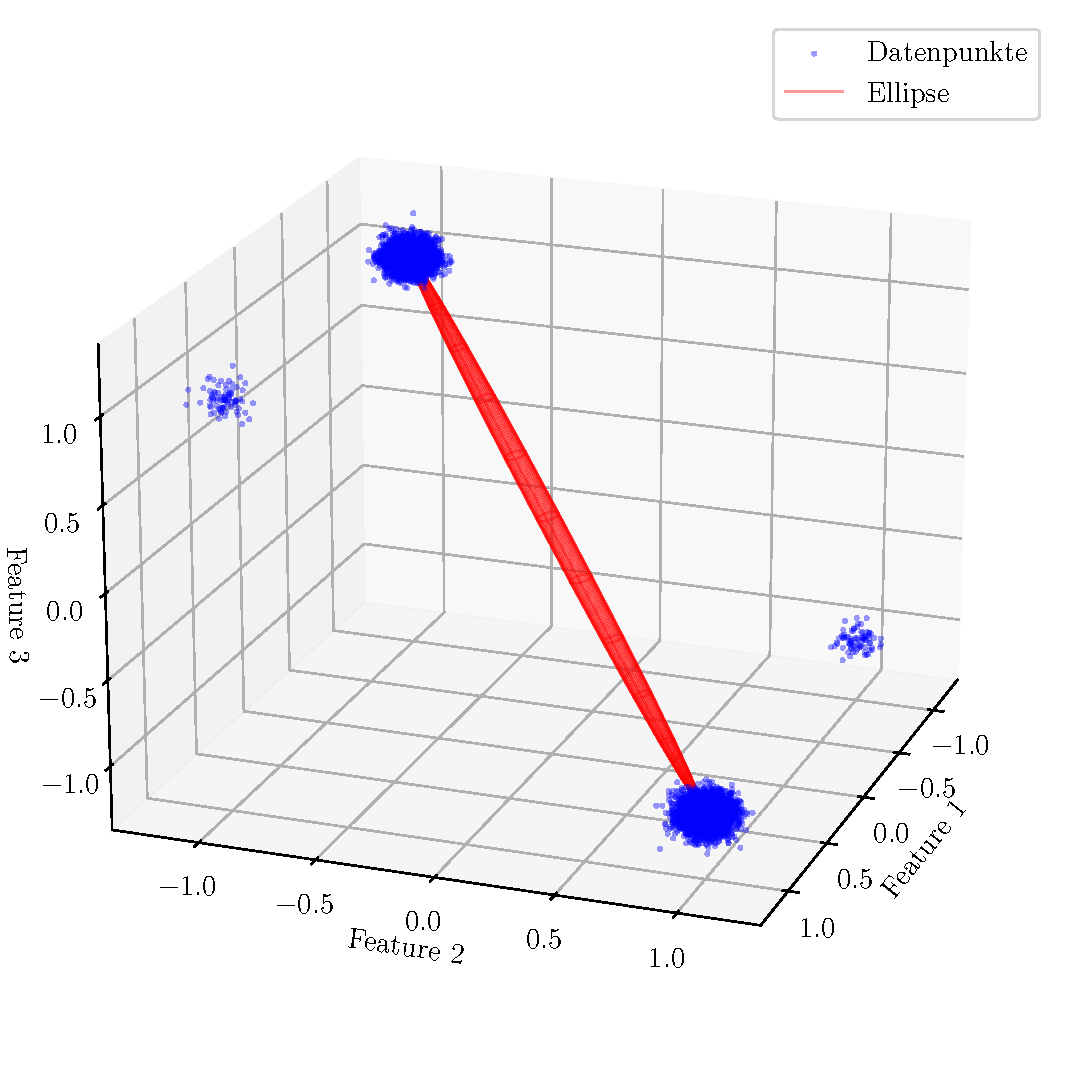
\includegraphics[width=1\linewidth]{ch4_anomalien/abbildungen/EE_ellipse.pdf}
    \caption{Ellipsoid auf Basis der Kovarianz der drei Kanäle}
    \label{fig:ee_ellipse}
\end{figure}

\section{Semi-Supervised Learning Algorithmen}
Eine weitere Möglichkeit der Anomaliedetektion ist die mit Algorithmen der Klasse \textbf{Semi-Supervised Learning}. Algorithmen dieser Klasse benötigen
Trainingsdaten, die dem Normal entsprechen und sind daher zu Beginn der Implementierung zunächst unpraktischer als die der Klasse Unsupervised Learning.
Der Grund dafür ist, dass erst eine erhebliche Menge an Training durchgeführt werden muss, optimalerweise mit Daten, die den gesamten normalen Betriebsbereich
abdecken können~\cite[S.~2-4]{Chapelle2010}~\cite{Schmidl2022}. Dementsprechend werden Datenpunkte- oder sequenzen, die nicht dem Normal angehören oder
als solches identifiziert werden können, als Anomalie gekennzeichnet.

Das Sammeln von großen Datensätzen ist kein Problem. Das SSP X1 System nimmt beispielsweise im Sekundentakt Daten auf und so entstehen schnell große
Datensätze bzw.~Zeitserien. Die Problematik liegt vielmehr darin, dass die Daten mit einem Label versehen werden müssen, zumindest implizit. Es muss
sichergestellt sein, dass die gesamte vorliegende Zeitserie einem normalen Betriebszustand entspricht~\cite[S.~10~ff]{Chapelle2010}.

\subsection{LSTM-Autoencoder}
Einer in seiner Funktionalität interessanter Algorithmus ist der LSTM-Autoencoder (LSTM-AE). LSTM steht für Long-Short Term Memory, ist eine Erweiterung der
Recurrent Neural Networks und erlaubt es, auf ein Langzeitgedächtnis zurückzugreifen und kommt gänzlich ohne Parametrisierung aus~\cite{Hochreiter1997}.
Ein Autoencoder ist ein Algorithmus, der auf Basis der Rekonstruktion von Sequenzen Anomalien detektiert und gehört demnach zur Kategorie der
Subsequenzanomaliedetektion~\hyperref[tab:algorithmen]{(vgl.~Tab.~\Ref*{tab:algorithmen})}.

Die Einordnung in die Klasse der Rekonstruktionsalgorithmen erfolgt nach Schmidl et al.~\cite{Schmidl2022} und beschreibt Rekonstruktionsalgorithmen
als solche, die Subsequenzen in eine niederdimensionalere Do\-mäne enkodieren, von wo sie wieder dekodiert bzw.~rekonstruiert werden. Ein zu analysierender
Datensatz wird also in Subsequenzen unterteilt und diese werden enkodiert. Mithilfe der Trainingsdaten werden die enkodierten Sequenzen rekonstruiert,
wobei Abweichungen des Originals zur rekonstruierten Sequenz als Anomalie gelten dürfen, da sie mit den Trainingsdaten nicht übereinstimmen.

Die Kombination der beiden Prinzipien zum LSTM-AE erlaubt die Enkodierung der Subsequenzen unter Beibehalt langzeitiger Abhängigkeiten und Korrelationen
und erweist sich so als sehr geeignet für große multivariate Zeitserien mit unterschiedlichen Abhängigkeiten und Korrelationen, wie sie in den Systemen
der SSP X1 vorkommen~\cite{Wei2022}.

Der Algorithmus wird im nächsten Kapitel denselben Tests unterzogen wie seine Unsupervised Learning Pendants. Schlussendlich ist auch eine
Implementierung von LSTM-AE zur Anomaliedetektion im Kontext der SSP X1 und verwandter Systeme nicht auszuschließen.

\section{Übersicht über alle ausgewählten Algorithmen}

Abschließend folgt eine kurze Auflistung aller genannten Algorithmen mit stichwortartiger Kategorisierung nach Detektionsklasse, -prinzip sowie die Quelle der
Implementierung. Unter dem Stichwort \textit{Eigene Implementierung} verbergen sich auch Komponenten, die aus Python Bibliotheken angewandt wurde, wie der
Algorithmus zu \textbf{Isolation Forest}~\cite{scikit-learn}, die zur gewollten Funktionalität
zusammengeführt und erweitert wurden. Im nächsten Kapitel erfolgt die Erprobung, Gegenüberstellung und Evaluierung sämtlicher Algorithmen derselben
Detektionsklasse.

\begin{table}[h]
    \renewcommand{\arraystretch}{1.75}
    \begin{tabular}{c||c|c|c}
\textbf{Algorithmus}                        & \textbf{Detektionsklasse}     & \textbf{Detektionsprinzip}   & \textbf{Quelle}               \\
\hline
\textbf{HBOS}                               & Punktanomalien        & Histogramm          & PyOD (Open Source)~\cite{zhao2019pyod}     \\
\hline
\multirow{2}{*}{\textbf{Sliding Window}}    & \multirow{2}{*}{Punktanomalien}        & \multirow{2}{*}{Z-Score} & \multirow{2}{*}{Eigene Implementierung} \\
\textbf{Z-Score} & & & \\
\hline
\textbf{GrammarViz 2.0}                     & Subsequenzanomalien   & Grammatik           & Open Source~\cite{senin-gv2}           \\
\hline
\textbf{SWIFD}                              & Subsequenzanomalien   & Isolation Tree      & Eigene Implementierung     \\
\hline
\multirow{2}{*}{\textbf{MD-SWIFD}}          & \multirow{2}{*}{Korrelationsanomalien} & \multirow{2}{*}{Mahalanobis Distanz} & \multirow{2}{*}{Eigene Implementierung} \\
 & & und Isolation Tree & \\
\hline
\multirow{2}{*}{\textbf{Elliptic Envelope}} & \multirow{2}{*}{Korrelationsanomalien} & \multirow{2}{*}{Kovarianzmatrix und} & \multirow{2}{*}{sklearn (Open Source)~\cite{scikit-learn}} \\
 & & Mahalanobis Distanz & \\
\hline\hline
\multirow{2}{*}{\textbf{LSTM-AE}}           & \multirow{2}{*}{Subsequenzanomalien}   & \multirow{2}{*}{Rekonstruktion und} & \multirow{2}{*}{Open Source~\cite{pytorch-LSTMAE}} \\
 & & Neuronale Netze &
\end{tabular}
    \caption{\centeringÜbersicht über die verwendeten Algorithmen nach Kategorisierung in Detektionsklasse, Detektionsprinzip und Ursprung}
~\label{tab:algorithmen}
\end{table}